\documentclass{article}
\usepackage{graphicx} % Required for inserting images
\usepackage{amsmath}
\usepackage{hyperref}

\title{Centrality Metrics in Graph Node Networks}
\author{By: Gargie Tambe, Asish Bharadwaj, Chetan Vellanki}

\date{June 2023}

\begin{document}

\maketitle

\section*{Introduction}
Centrality measures play a critical role in the field of graph analytics as they provide valuable insights into the importance and influence of individual nodes within a network. By quantifying the centrality or "centrality" of nodes, researchers can identify key entities that have a significant impact on network dynamics, control the flow of information, or act as vital connectors within the network structure.

\begin{center}
    \includegraphics[scale=0.25]{graph.png}  
\end{center}

The concept of centrality encompasses multiple perspectives, allowing researchers to evaluate the significance of nodes from various angles. This versatility is particularly valuable, as it enables the analysis of complex systems such as human brain networks or social networks, where understanding the role and importance of individual nodes is crucial for comprehending the overall system dynamics.

This review aims to explore and evaluate the key characteristics and limitations of commonly used centrality measures, focusing on Degree Centrality, Betweenness Centrality, and Eigenvector Centrality. Additionally, we will demonstrate how centrality measures can be effectively combined with linear algebraic concepts to gain a deeper understanding of the operation and behavior of complex systems.

Furthermore, we will delve into real-world scenarios and practical applications of centrality analysis, showcasing how these measures have been successfully utilized in diverse fields such as social network analysis, disease spread modeling, recommendation systems, and urban planning.

\section*{Types of Centrality Metrics}

\begin{itemize}

\item \textbf{Degree Centrality}

Degree centrality is a fundamental measure in network analysis that quantifies the importance of a node within a graph based on its degree, which represents the number of connections it has to other nodes. It serves as a simple and intuitive indicator of node prominence, with nodes having a higher degree of centrality considered more central or influential in the network. Degree centrality is widely used in various domains, including social network analysis, transportation networks, and biological networks, providing valuable insights into key nodes and network structure. By considering the immediate connections of a node, degree centrality offers a valuable perspective on node importance without implying any negative connotations.

In a given graph $G(V, E)$, for a given vertex $v$, the degree centrality is defined as the following -

$$ C_{D}(v) = deg(v) $$

Time complexity: Calculating the degree centrality for all nodes in a graph, it takes $\Theta(V^{2})$ time in a dense adjacency matrix and for edges, $\Theta(E)$ time in a sparse matrix representation.

Let $X(Y,Z)$ be the $|Y|$ node connected graph, with $|Y|$ vertices and $|Z|$ edges, that maximizes the following quantity (where $y*$ is node with highest degree centrality in $|X|$:

$$ H = \sum_{j = 1}^{|Y|} [C_{D}(y*) - C_{D}(y_{j})]$$

So, the degree centrality of the graph $G$ will be:

$$ C_{D}(G) = \frac{\sum_{i=1}^{|V|}[C_{D}(v*) - C_{D}(V_i)]}{H} $$

The value of H is maximized when graph $X$ contains one central node to which all other nodes are connected (star topology). In that case, 

$$H = (n-1) \times ((n-1)-1) = n^{2}-3n+2 $$

Let's consider the following graph - 

\begin{center}
    \includegraphics[scale=0.3]{dc.png}
\end{center}

The degree of each of the nodes would be as follows -

\begin{center}
\begin{tabular}{|c|c|}
    \hline
    Node & Degree \\
    \hline
    1 & 2 \\
    2 & 3 \\
    3 & 3 \\
    4 & 3 \\
    5 & 3 \\
    \hline
\end{tabular}
\end{center}

Code in Python for calculating Degree Centrality -

\begin{verbatim}
    import networkx as nx
    import matplotlib.pyplot as plt
    
    G = nx.Graph([(1, 2), (1, 3), (1, 4), (2, 3), (2, 4)])
    nx.draw(G, with_labels=True)
    nx.degree_centrality(G)
\end{verbatim}

Output would be -

\begin{verbatim}
    {1: 0.5, 3: 0.75, 4: 0.75, 2: 0.75, 5: 0.75}
\end{verbatim}

By utilising this metric, it is possible to identify influential individuals in a network, including those with the most extensive contact networks, those transitioning rapidly between peers, and those with access to the most essential information.

\item \textbf{Betweenness Centrality}

Betweenness centrality is a metric that assesses the significance of a node in a network based on its frequency in the geodesic distance or shortest path between all pairs of nodes. It identifies nodes that serve as connectors between distinct groups within the network, playing a pivotal role in controlling the flow of interactions or information. Although originating from social network analysis, betweenness centrality finds applicability in various network types, including social, transportation, and computer networks.

The betweenness centrality of a vertex v in a graph can be calculated using the following formula, which involves linear algebra:

$$ BC(v) = \sum_{u, v\ \epsilon \ V} \frac{\sigma_{uw}(v)}{\sigma_{uw}}$$

where V represents the set of all nodes in the graph, $\sigma_{uw}$ denotes the total number of shortest paths between node $u$ and $v$, and $\sigma_{uw}(v)$ is the total number of shortest paths between nodes $u$ and $w$ that pass through vertex $v$.

Following steps are followed to calculate the betweenness centrality of a vertex v in a graph -
\begin{enumerate}
    \item Calculate unique pairs of nodes (unique edges):     
    Start by considering all possible pairs of nodes in the graph. These pairs represent the edges or connections between nodes.
    \item Determine the shortest paths:
    Find the shortest paths between all pairs of nodes in the graph. This can be done using algorithms such as Dijkstra's algorithm or Floyd-Warshall algorithm. In case of a weighted graph, the paths should be minimal weighted paths.
    \item Calculate the sum of all fractions of shortest paths through vertex v:
    For each pair of nodes $(u,w)$ calculate the number of shortest paths between them ($\sigma_{uw}$) and the number of paths that pass through the vertex v ($\sigma_{uw}(v)$). Then, sum up the fractions $\frac{\sigma_{uw}}{\sigma_{uw}(v)}$ for all pairs of nodes in which vertex $v$ lies on the shortest path.
    \item Normalize the betweenness centrality (BC): 
    If you are comparing networks of different sizes, it is common practice to normalize the betweenness centrality scores. This normalization takes into account the fact that larger networks tend to have higher centrality scores. There are various normalization techniques, such as dividing each node's betweenness centrality by the maximum possible betweenness centrality value.
\end{enumerate}

Let's consider the following example to calculate Betweenness Centrality,

\begin{center}
    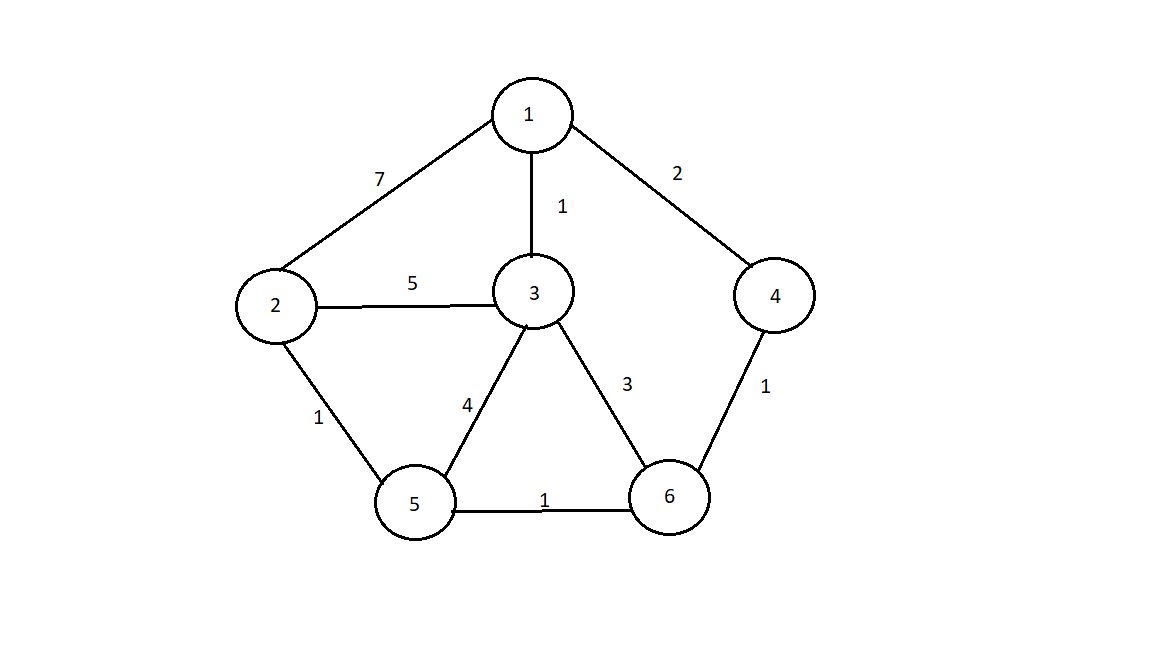
\includegraphics[scale=0.20]{bc.png}  
\end{center}

Pseudocode to find Betweenness Centrality -

\begin{verbatim}
function betweenness_centrality(graph):
    for each node in the graph:
        // Initialize
        shortest_paths_count = {}
        dependency = {}
        stack = {}
        distance = {}
        num_shortest_path = {}

        // BFS to find shortest path in the graph and to count number of
        shortest paths
        distance[node] = 0
        num_shortest_paths[node] = 1

        queue = {}
        enqueue(queue, node)
        while the queue is not empty:
            current_node = dequeue(queue)
            push(stack, current_node)

            for each neighbour in neighbours(current_node):
                if neighbour is not visited:
                    mark neighbour as visited 
                    enqueue(queue, neighbour)
                    distance[neighbor] = distance[current_node] + 
                    edge_weight(current_node, neighbor)
                    num_shortest_paths[neighbor] = num_shortest_paths[neighbor] 
                    + num_shortest_paths[current_node]

        for each node in the graph:
            dependency[node] = 0.0

        // Calculate dependency values
        while stack is not empty:
            current_node = pop(stack)

            for each neighbor in neighbors(current_node):
                if distance[neighbor] = distance[current_node] +
                edge_weight(current_node, neighbor):
                    dependency[neighbor] = dependency[neighbor] + 
                    (num_shortest_paths[neighbor] / 
                    num_shortest_paths[current_node]) * 
                    (1 + dependency[current_node])

            betweenness[current_node] = betweenness[current_node] +
            dependency[current_node]

    // Normalize the betweenness centrality values 
    for each node in graph:
        betweenness[node] = betweenness[node] / ((graph_size - 1) * 
        (graph_size - 2))

    return betweenness
\end{verbatim}

Code in Python - 

\begin{verbatim}
    import networkx as nx
    import matplotlib.pyplot as plt 
    %matplotlib notebook

    G = nx.Graph()
    G.add_edge(1, 2, weight = 7)
    G.add_edge(1, 3, weight = 1)
    G.add_edge(1, 4, weight = 2)
    G.add_edge(2, 3, weight = 5)
    G.add_edge(5, 2, weight = 1)
    G.add_edge(3, 5, weight = 4)
    G.add_edge(3, 6, weight = 3)
    G.add_edge(5, 6, weight = 1)
    G.add_edge(4, 6, weight = 1)
    G.edges(data = True)

    nx.draw_networkx(G, with_labels = True)

    betweenness = nx.betweenness_centrality(G, weight = 'weight')
    print(betweenness)  
\end{verbatim}

Output - 

\begin{verbatim}
    {1: 0.1, 2: 0.0, 3: 0.0, 4: 0.30000000000000004, 
    5: 0.3666666666666667, 6: 0.4833333333333334}
\end{verbatim}

For example, in the given graph, the betweenness centrality would be as follows -

\begin{center}
\begin{tabular}{|c|c|c|c|}
    \hline
    Edge & $\sigma_{uw}$ & $\sigma_{uw}(v)$ & $\frac{\sigma_{uw}(v)}{\sigma_{uw}}$ \\
    \hline
    (1, 2) & 1 & 1 & 1 \\
    (1, 3) & 1 & 0 & 0 \\
    (1, 5) & 1 & 1 & 1 \\
    (1, 6) & 1 & 1 & 1 \\
    (2, 3) & 3 & 0 & 0 \\
    (2, 5) & 1 & 0 & 0 \\
    (2, 6) & 1 & 0 & 0 \\
    (3, 5) & 2 & 0 & 0 \\
    (3, 6) & 1 & 0 & 0 \\
    (5, 6) & 1 & 0 & 0 \\
    \hline
\end{tabular}    
\end{center}

Hence betweenness centrality of 4 is: 3

\begin{center}
\begin{tabular}{|c|c|c|c|}
    \hline
    Edge & $\sigma_{uw}$ & $\sigma_{uw}(v)$ & $\frac{\sigma_{uw}(v)}{\sigma_{uw}}$ \\
    \hline
    (1, 2) & 1 & 1 & 1 \\
    (1, 3) & 1 & 0 & 0 \\
    (1, 5) & 1 & 1 & 1 \\
    (1, 4) & 1 & 0 & 0 \\
    (2, 3) & 3 & 1 & 1/3 \\
    (2, 5) & 1 & 0 & 0 \\
    (2, 4) & 1 & 1 & 1 \\
    (3, 5) & 2 & 1 & 1/2 \\
    (3, 4) & 1 & 0 & 0 \\
    (5, 4) & 1 & 1 & 1 \\
    \hline
\end{tabular}    
\end{center}

Hence betweenness centrality of 6 is: 4.83

\begin{center}
\begin{tabular}{|c|c|c|c|}
    \hline
    Edge & $\sigma_{uw}$ & $\sigma_{uw}(v)$ & $\frac{\sigma_{uw}(v)}{\sigma_{uw}}$ \\
    \hline
    (1, 2) & 1 & 1 & 1 \\
    (1, 3) & 1 & 0 & 0 \\
    (1, 4) & 1 & 0 & 0 \\
    (1, 6) & 1 & 0 & 0 \\
    (2, 3) & 3 & 2 & 2/3 \\
    (2, 4) & 1 & 1 & 1 \\
    (2, 6) & 1 & 1 & 1 \\
    (3, 4) & 1 & 0 & 0 \\
    (3, 6) & 1 & 0 & 0 \\
    (4, 6) & 1 & 0 & 0 \\
    \hline
\end{tabular}    
\end{center}

Hence betweenness centrality of 5 is: 3.67

\begin{center}
\begin{tabular}{|c|c|c|c|}
    \hline
    Edge & $\sigma_{uw}$ & $\sigma_{uw}(v)$ & $\frac{\sigma_{uw}(v)}{\sigma_{uw}}$ \\
    \hline
    (1, 4) & 1 & 0 & 0 \\
    (1, 3) & 1 & 0 & 0 \\
    (1, 5) & 1 & 0 & 0 \\
    (1, 6) & 1 & 0 & 0 \\
    (4, 3) & 1 & 0 & 0 \\
    (4, 5) & 1 & 0 & 0 \\
    (4, 6) & 1 & 0 & 0 \\
    (3, 5) & 2 & 0 & 0 \\
    (3, 6) & 1 & 0 & 0 \\
    (5, 6) & 1 & 0 & 0 \\
    \hline
\end{tabular}    
\end{center}

Hence betweenness centrality of 2 is: 0

\begin{center}
\begin{tabular}{|c|c|c|c|}
    \hline
    Edge & $\sigma_{uw}$ & $\sigma_{uw}(v)$ & $\frac{\sigma_{uw}(v)}{\sigma_{uw}}$ \\
    \hline
    (1, 2) & 1 & 0 & 0 \\
    (1, 4) & 1 & 0 & 0 \\
    (1, 5) & 1 & 0 & 0 \\
    (1, 6) & 1 & 0 & 0 \\
    (2, 4) & 1 & 0 & 0 \\
    (2, 5) & 1 & 0 & 0 \\
    (2, 6) & 1 & 0 & 0 \\
    (4, 5) & 2 & 0 & 0 \\
    (4, 6) & 1 & 0 & 0 \\
    (5, 6) & 1 & 0 & 0 \\
    \hline
\end{tabular}    
\end{center}

Hence betweenness centrality of 3 is: 0

\begin{center}
\begin{tabular}{|c|c|c|c|}
    \hline
    Edge & $\sigma_{uw}$ & $\sigma_{uw}(v)$ & $\frac{\sigma_{uw}(v)}{\sigma_{uw}}$ \\
    \hline
    (4, 2) & 1 & 0 & 0 \\
    (4, 3) & 1 & 1 & 0 \\
    (4, 5) & 1 & 0 & 0 \\
    (4, 6) & 1 & 0 & 0 \\
    (2, 3) & 3 & 0 & 0 \\
    (2, 5) & 1 & 0 & 0 \\
    (2, 6) & 1 & 0 & 0 \\
    (3, 5) & 2 & 0 & 0 \\
    (3, 6) & 1 & 0 & 0 \\
    (5, 6) & 1 & 0 & 0 \\
    \hline
\end{tabular}    
\end{center}

Hence betweenness centrality of 1 is: 1

Maximum possible betweenness centrality for an undirected graph (M) is:

$$\frac{(N-1)\times(N-2)}{2} = \frac{(6-1)\times(6-2)}{2} = 10$$

\begin{center}
\begin{tabular}{|c|c|c|}
    \hline
    Vertex & Betweenness Centrality & Normalized BC ( = BC/M) \\
    \hline
    1 & 1 & 0.1 \\
    2 & 0 & 0 \\
    3 & 0 & 0 \\
    4 & 3 & 0.3 \\
    5 & 3.67 & 0.367 \\
    6 & 4.83 & 0.483 \\
    \hline
\end{tabular}    
\end{center}

The betweenness centrality metric provides a unique perspective on the significance of nodes compared to other centrality measures. It focuses on individuals who have control over the flow of data throughout the network, including brokers, controllers, intermediaries, gatekeepers, and similar roles. Removing nodes with high betweenness centrality from the network would have the most disruptive impact on the interactions within the network.

\item \textbf{Eigenvector Centrality}

Eigen Vector Centrality is a metric that assesses the importance of nodes in a graph based on their connections to highly important nodes. It assigns scores to nodes, considering that a node contributes more to its score if it is connected to other nodes with high scores. This measure is calculated using an iterative algorithm that converges to stable scores. Eigenvector Centrality is used in various domains, such as social network analysis, biology, and recommendation systems, to identify influential nodes within a network.

The Eigenvector Centrality (EVC) of a node in a network can be computed using the adjacency matrix of the network. 

For a graph $G(V, E)$ where $|V|$ is the number of vertices of the graph network.  $A = (a_{v,t})$ is the adjacency matrix of the graph. $ a_{v,t} = 1 $ if there exists an edge between vertex $v$ and vertex $t$ and $ a_{v,t} = 0 $, otherwise. 

The formula for calculating EVC is as follows:

$$ x_{v} = \frac{1}{\lambda} \sum_{t \epsilon M(v)} x_{t} = \frac{1}{\lambda} \sum_{t \epsilon G } a_{v,t}x_{t} $$

where $M(v)$ is the set of neighbours of $v$ and $\lambda$ is the eigenvalue. 

Multiplying both LHS and RHS by $\lambda$ on both sides, we see that $\sum_{t \epsilon G} a_{v,t}x_{t}$ is the product of the adjacency matrix A with the vector $v$ i.e. $Ax$. The LHS part of the product of vector $x$, i.e. $\lambda x$.

Rearranging, we get, $Ax = \lambda x$.

\end{itemize}

\section*{Applications and Related Works}

\begin{itemize}

\item Degree centrality analysis in social networking plays a pivotal role in understanding the structure and dynamics of social relationships. By measuring the number of connections a node has in a network, degree centrality provides insights into individual popularity, influence, and information dissemination potential. It helps identify influential hubs, brokers, and opinion leaders who serve as bridges between different communities, facilitating the spread of ideas and social influence. Conversely, it highlights individuals who may be isolated or peripheral, offering insights into barriers to information diffusion and social integration. Overall, degree centrality analysis informs marketing strategies, community engagement initiatives, and interventions aimed at understanding and leveraging social network dynamics.

\item Betweenness centrality has diverse applications, and one notable use case is in the analysis of criminal or terrorist networks. Nodes with high betweenness centrality in such networks often indicate crucial or highly involved actors. These nodes exert control over the flow of data among different groups, serving as bridges for information dissemination. Nodes with high betweenness centrality hold favorable positions in the network, facilitating greater control over information propagation. As a consequence, they become potential single points of failure. Disrupting or removing these nodes can effectively hinder communication and disrupt the network's operations.

\item The PageRank algorithm incorporates Eigen Vector Centrality as a fundamental element and is extensively employed by major companies, including Google, for website ranking purposes. By considering the World Wide Web as a directed graph, the algorithm evaluates the significance of web pages based on the quantity and quality of incoming links. Eigen Vector Centrality, leveraging eigenvectors and eigenvalues, iteratively computes centrality scores for web pages, ultimately establishing a ranking system that assigns priority to influential pages. This algorithmic application has brought about a paradigm shift in web search, enabling the provision of more accurate and pertinent search results to users, thereby enhancing their search experience.

\end{itemize}

\section*{References}

\begin{itemize}
    \item \href{https://www.works.so/blog/developers/centrality-metrics-for-graphs}{Centrality Metrics for Graphs - Works Blog}
    \item \href{https://www.turing.com/kb/graph-centrality-measures}{Graph Centrality Measures: Types and Explanation - Turing}
    \item \href{https://en.wikipedia.org/wiki/Centrality}{Centrality - Wikipedia}
    \item \href{https://www.geeksforgeeks.org/eigenvector-centrality-centrality-measure/}{Eigenvector Centrality (Centrality Measure) - GeeksforGeeks}
    \item \href{https://www.geeksforgeeks.org/degree-centrality-centrality-measure/}{Degree Centrality (Centrality Measure) - GeeksforGeeks}
    \item \href{https://www.geeksforgeeks.org/betweenness-centrality-centrality-measure/}{Betweenness Centrality (Centrality Measure) - GeeksforGeeks}
\end{itemize}

\section*{Work Contribution}

\begin{itemize}
    \item Gargie Tambe: Worked on Degree Centrality and designed the mid-report. 
    \item Asish Bharadwaj: Worked on Betweenness Centrality
    \item Chetan Vellanki: Worked on Eigen-Vector Centrality
\end{itemize}

\end{document}
